\chapter{Extra afbeeldingen, schema's \& code}
\label{app:A}
\section{Omzetting SQL naar NoSQL}
\begin{center}
\hvFloat[
%floatPos=h,
nonFloat=true,
capWidth=1,%
capPos=b,%
rotAngle=0,%
objectPos=c%
]{figure}{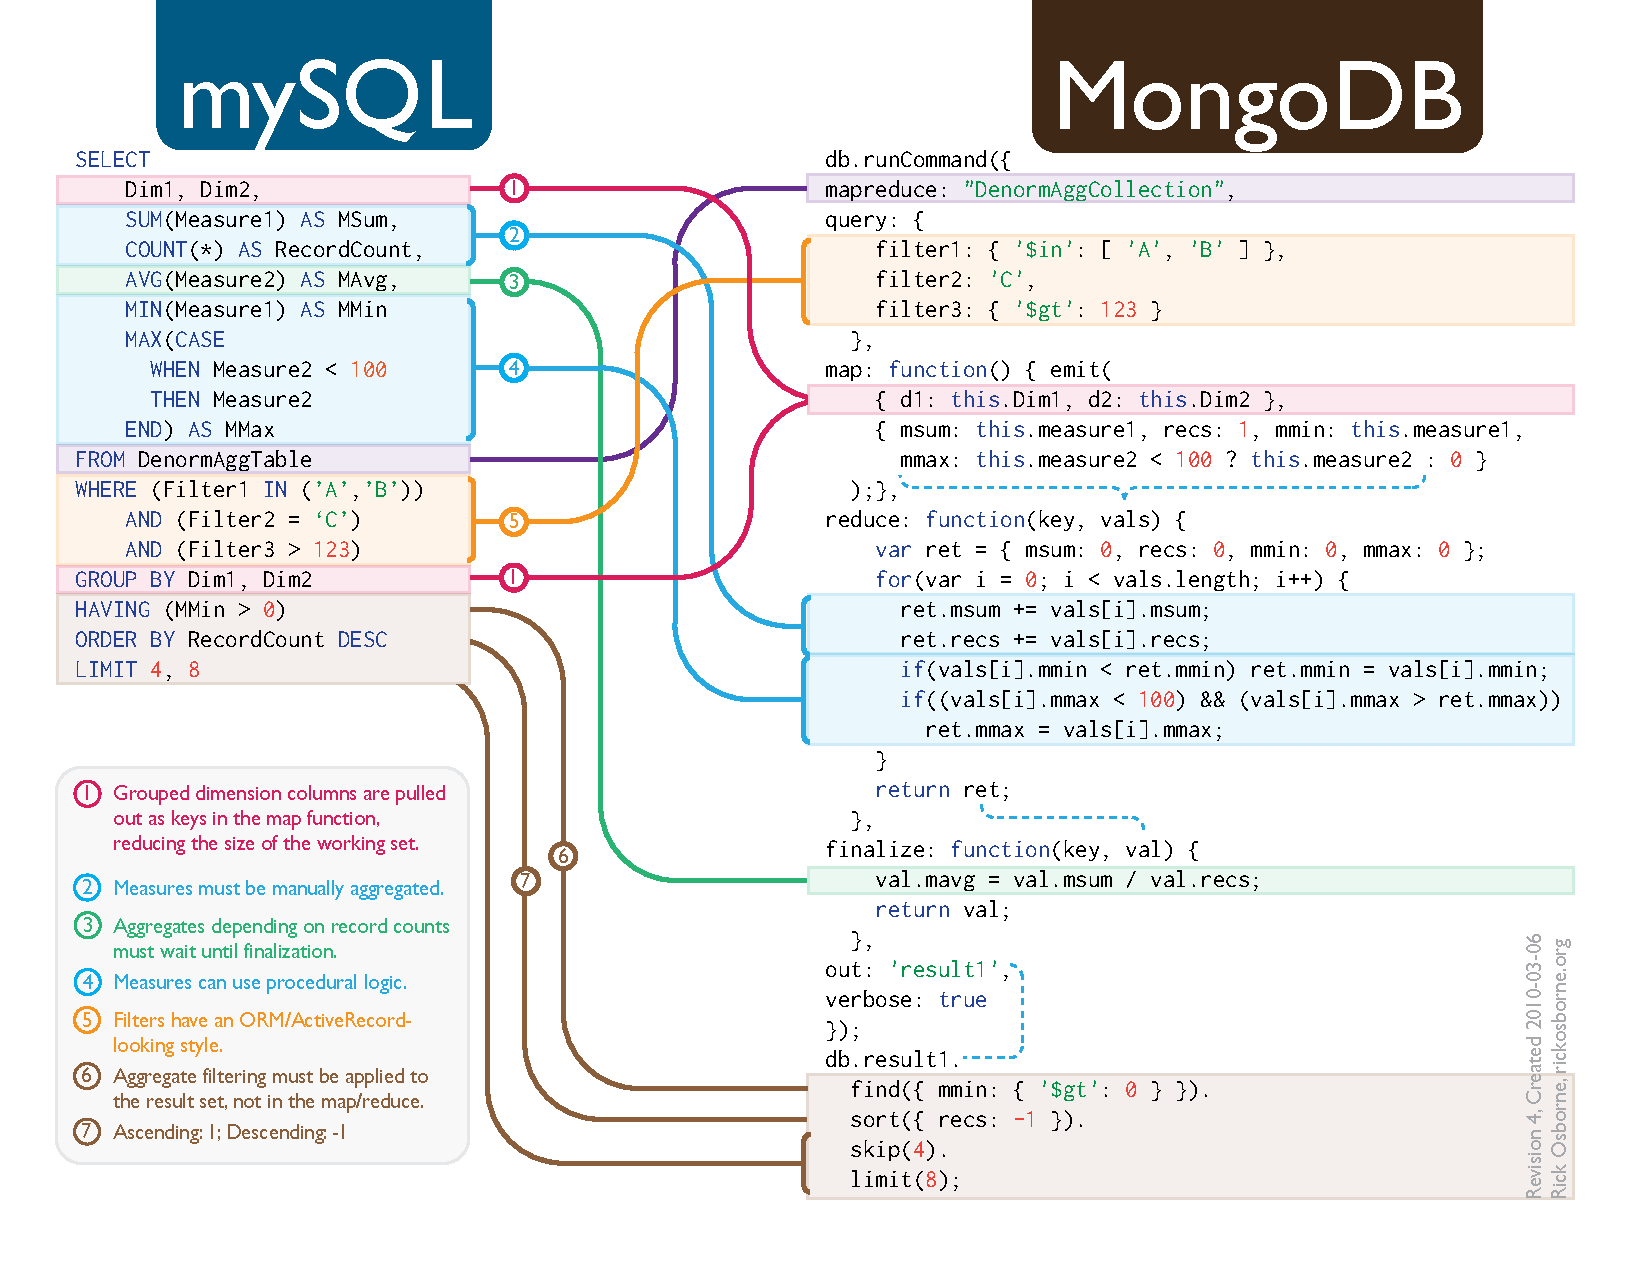
\includegraphics[width=0.6\textheight]{images/SQL-to-MongoDB.pdf}}{Sommige NoSQL systemen --- zoals MongoDB --- beschikken over dezelfde analytische kracht als een SQL database. De performantiekarakteristieken zijn echter verschillend. Afbeelding gebruikt met toestemming~\cite{sqlnosql}}{fig:sqlmongo}
\end{center}
%\clearpage
\pagebreak

%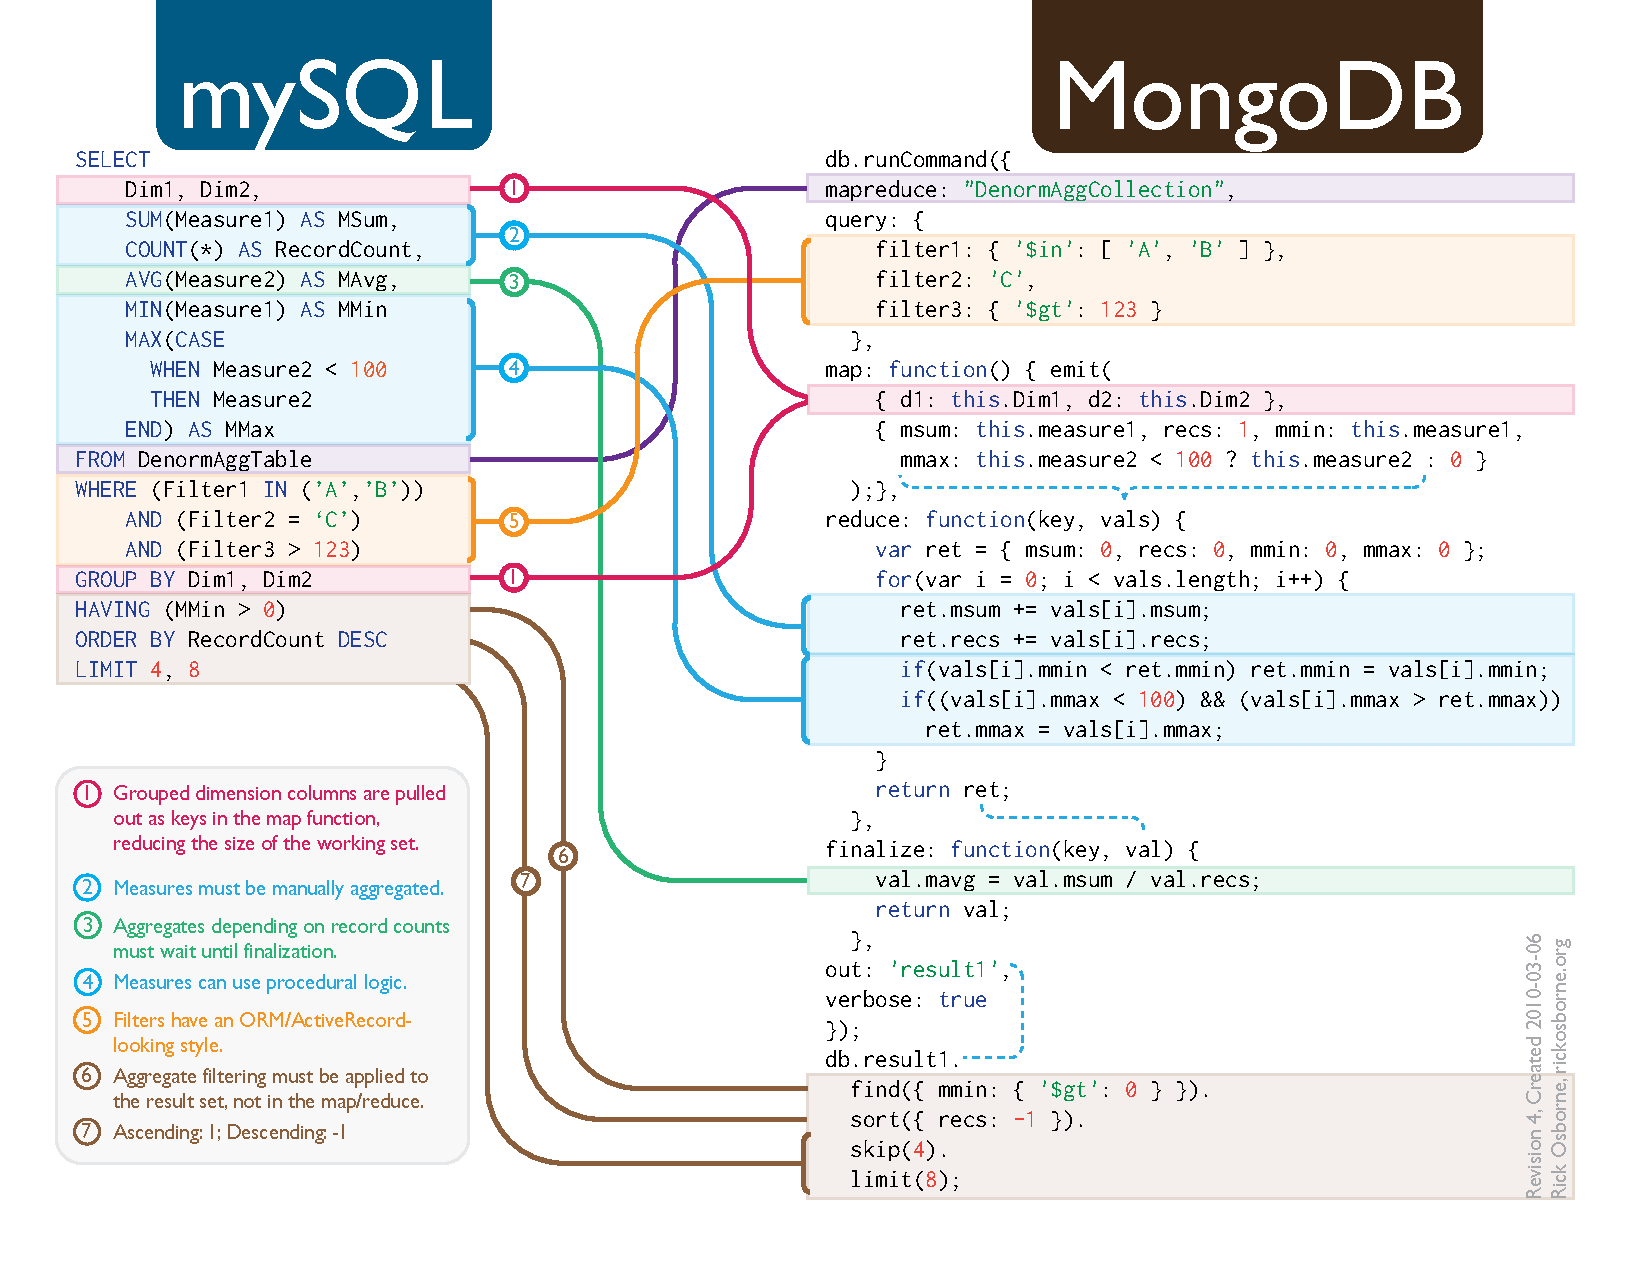
\includegraphics[width=0.8\textheight]{images/SQL-to-MongoDB.pdf}
%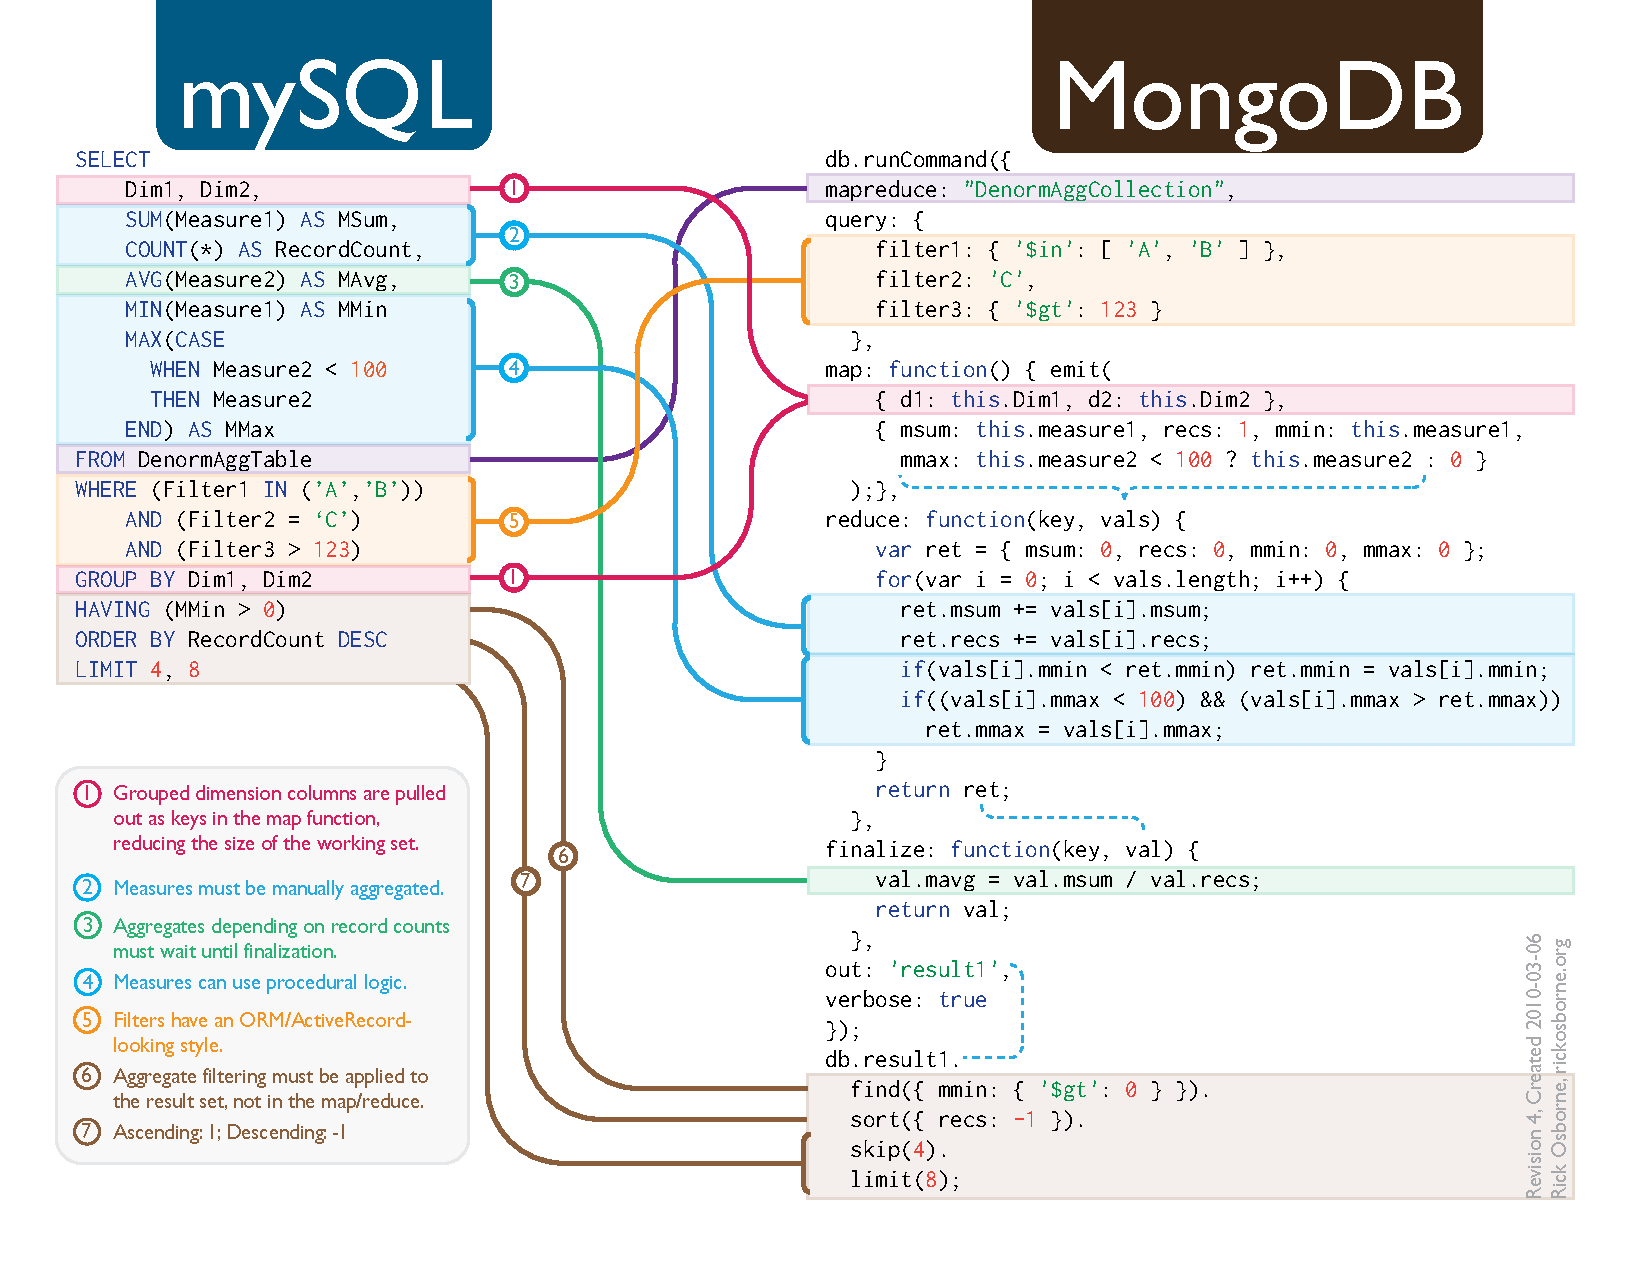
\includepdf{images/SQL-to-MongoDB.pdf}

\section{Overzicht van de applicatie}
\hvFloat[
%floatPos=h,
nonFloat=true,
capWidth=1,%
capPos=b,%
rotAngle=90,%
objectPos=c%
]{figure}{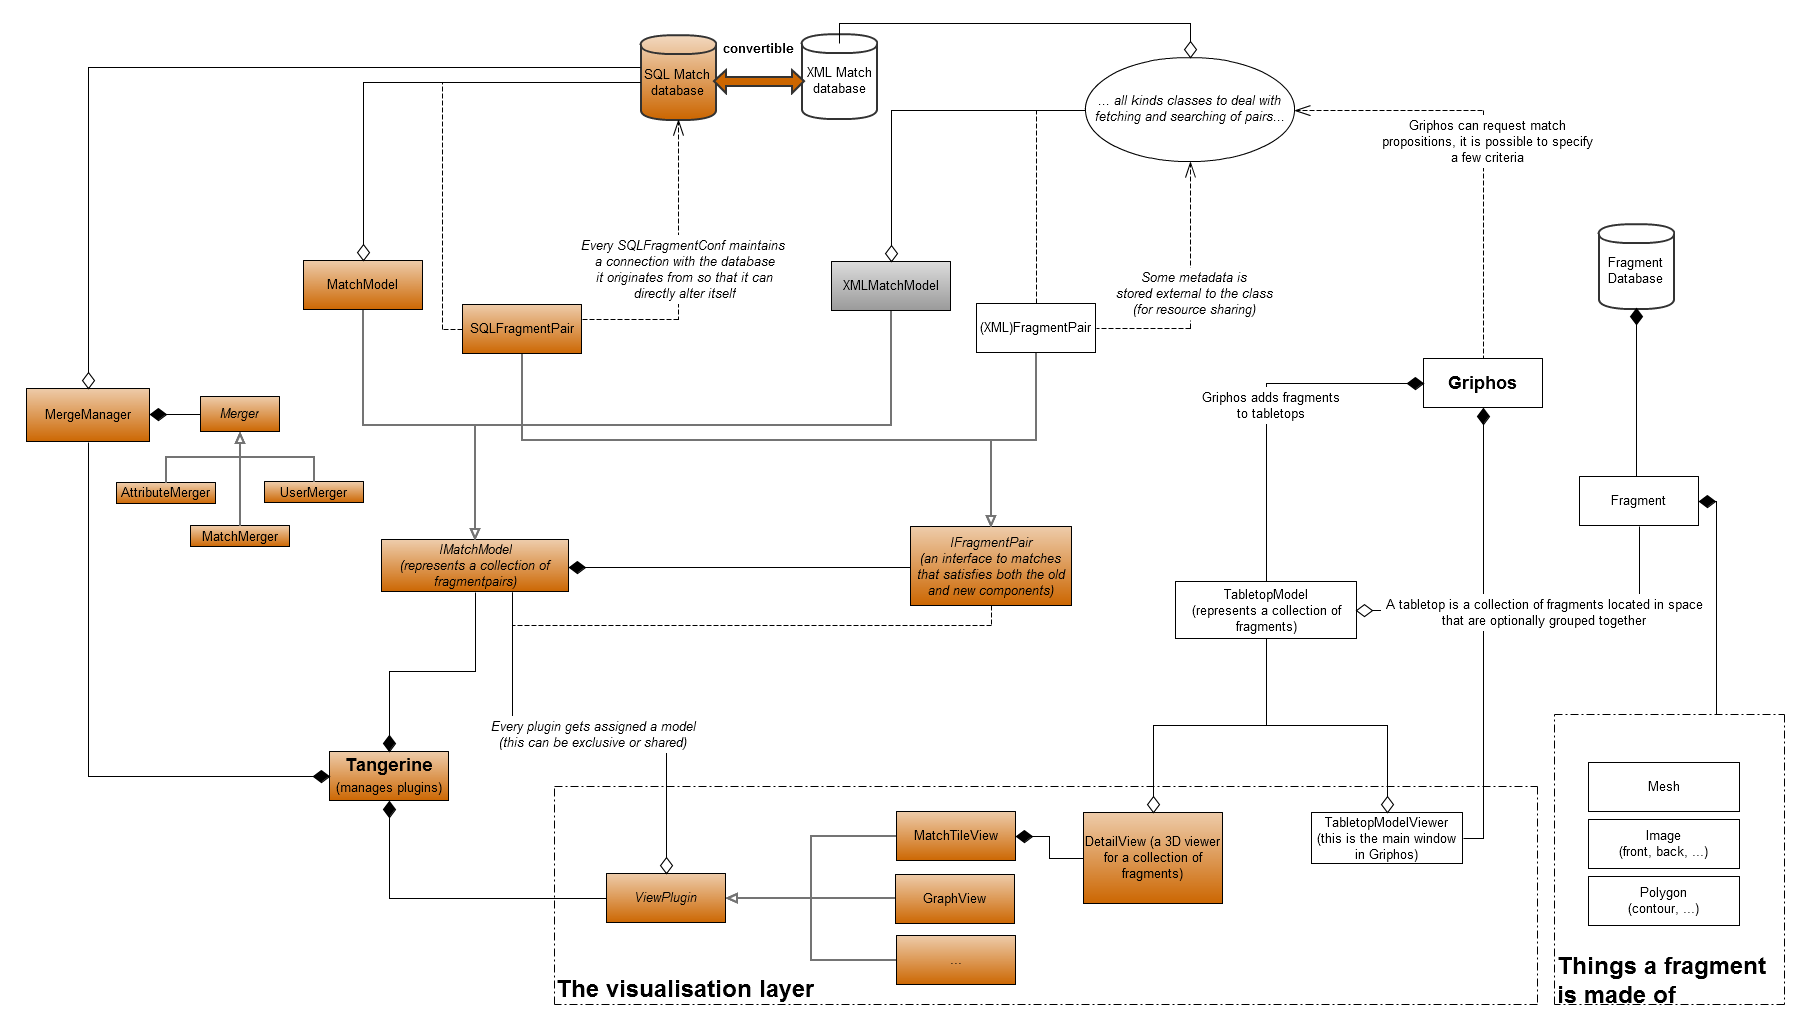
\includegraphics[width=0.95\textheight]{images/Bigtang.png}}{Een ruw overzicht van de componenten in het project en hoe het interageert met het reeds bestaande systeem.}{fig:tangbig}
\clearpage

\section{Detail van de synchronisatiestructuur}
\hvFloat[
%floatPos=h,
nonFloat=true,
capWidth=1,%
capPos=b,%
rotAngle=0,%
objectPos=c%
]{figure}{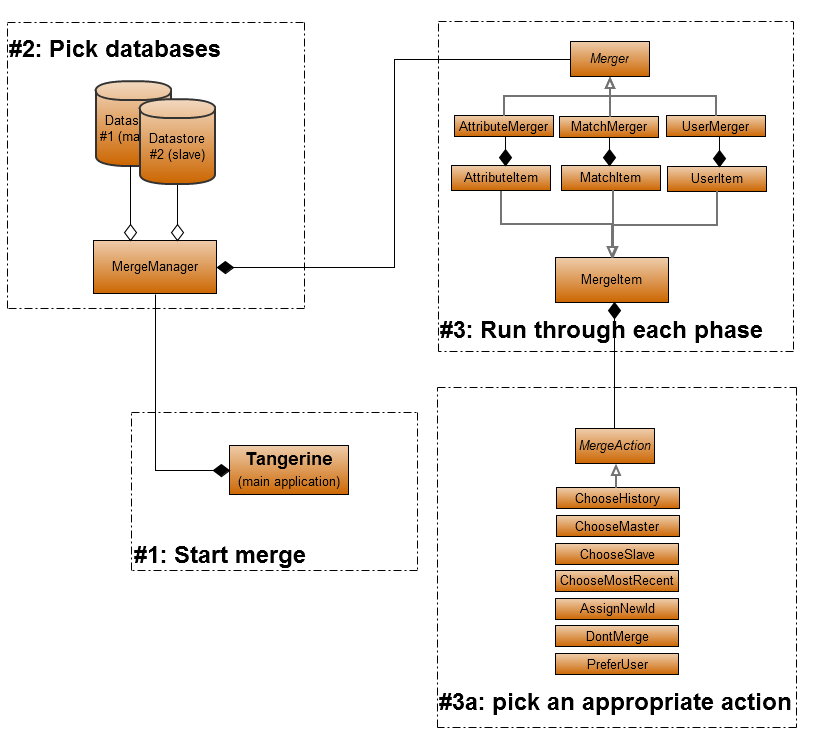
\includegraphics[width=\textwidth]{images/Overview-merging.png}}{Het synchronisatie-subsysteem, de componenten die overeenkomen met de stappen zijn aangeduid.}{fig:merging-overview}

\section{Graafqueries in SQL}

\lstinputlisting[label=code:sqlneigh,caption=SQL declaraties om een subgraaf van de collectie met bepaalde eigenschappen te extraheren, language=SQL]{source/findneighbours.sql}